\subsection{Instances}\label{sec:instances}
To investigate the problem we consider each flight as a vertex of a graph and
each conflict between two flights as an edge of this graph.  The connected
components of this \emph{conflict graph} represent natural subsets of the
problem. Figure~(\ref{fig:hist_cc}) shows the number of connected components by
varying the maximum delay time (Left), as well as the probability distribution
of the number of flights in each connected component. Interestingly, the large
part of connected components have small number of flights (for instance, $~75\%$
of the connected components for a maximum delay of $60$ minutes have no more
than $10$ flights). 

\begin{figure*}[t!]
  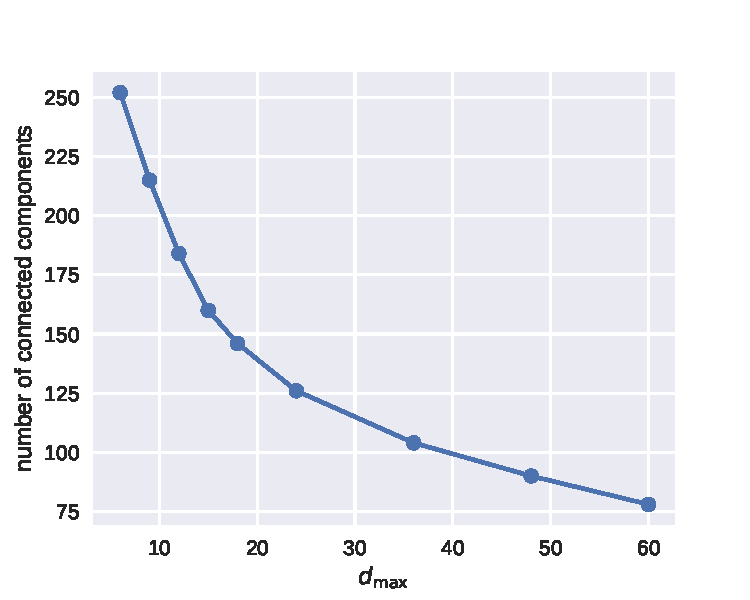
\includegraphics[width=\columnwidth]{pics/instances/num_cc.pdf}
  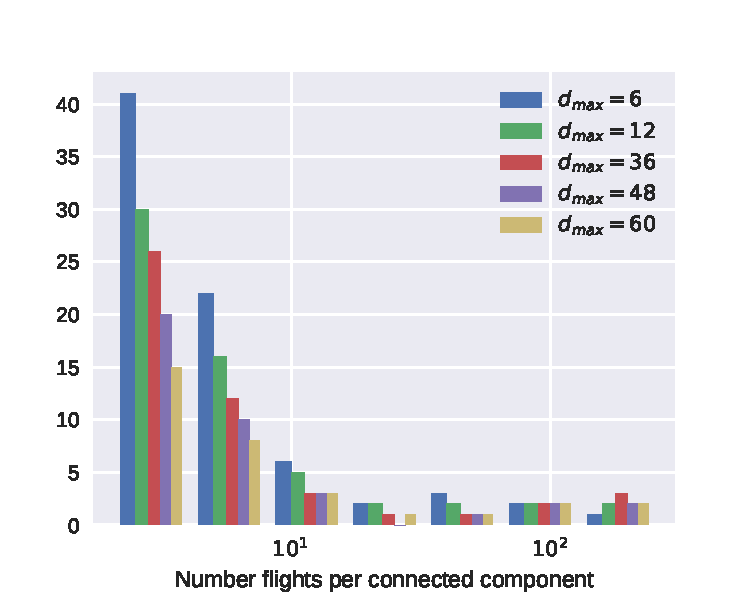
\includegraphics[width=\columnwidth]{pics/instances/analysis_cc.pdf}
  \caption{\label{fig:hist_cc}(Left) Number of connected components by varying
  the maximum delay time. (Right) Histogram of the number of flights inside a
  connected component, regardless the maximum delay time.}
\end{figure*}

As part of our analysis, we also studied the probability
distribution of the connectivity, namely the number of flights
for which a given flight share a potential conflict with. It is well known that
graphs with a non-trivial (small-world) structure with ``hubs'' have a
connectivity distribution which follows a power-law distribution
\cite{barabasi:99}. In the left panel of Figure~(\ref{fig:pl_cc}), we show the
connectivity distribution for a given maximum delay of $60$ minutes. As one can
see, the connectivity distribution shows a power-law decay of the form
$d^\alpha$, where $d$ is the connectivity of a given flight, indicating that 
the underlying topology of the ATM problem is not trivial. In the right panel of
Figure~(\ref{fig:pl_cc}) we also show the power-law decay $\alpha$ as a function
of the maximum delay time. As expected, $\alpha$ decreases by increasing the
maximum delay time. Indeed, the number of potential conflicts shared by two flights
increases as well by increasing the maximum delay time.\\

\begin{figure*}
  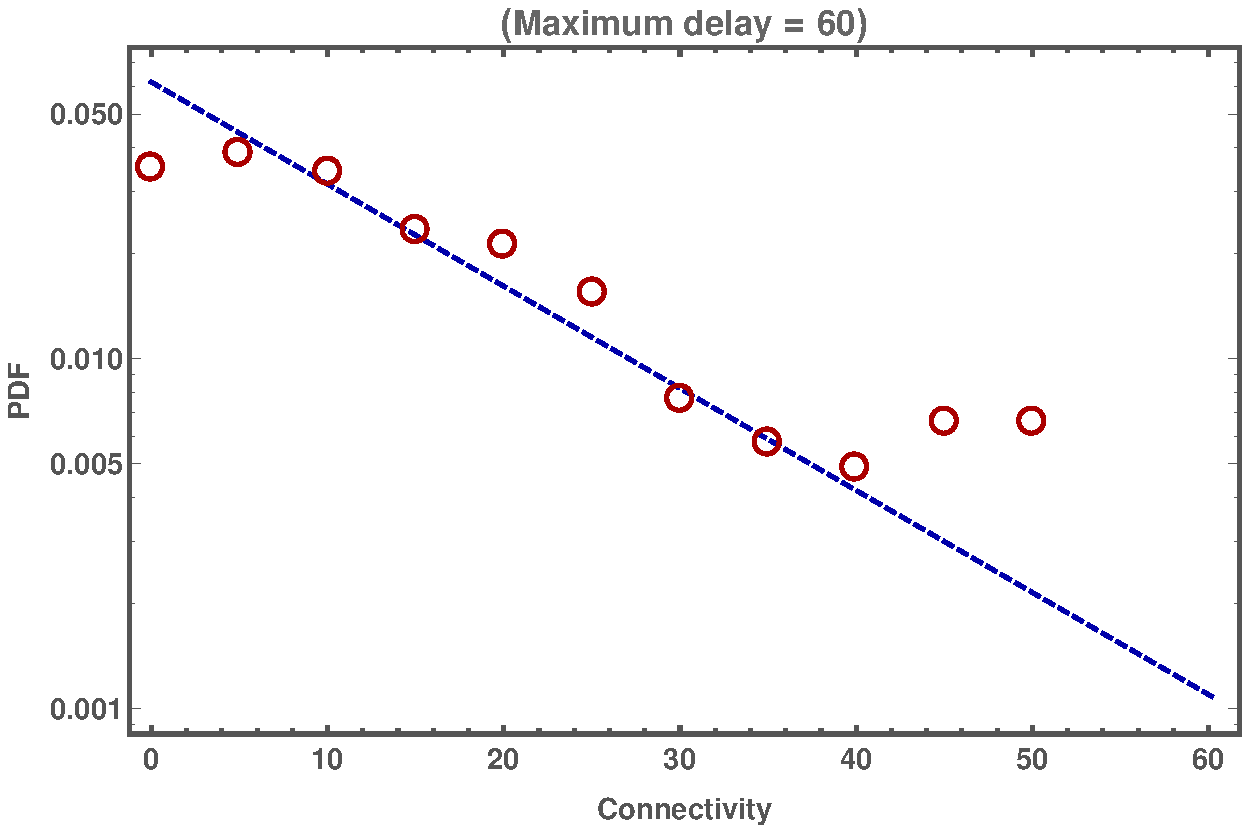
\includegraphics[width=0.95\columnwidth]{pics/instances/connectivity_pdf.pdf}
  \hspace{30pt}
  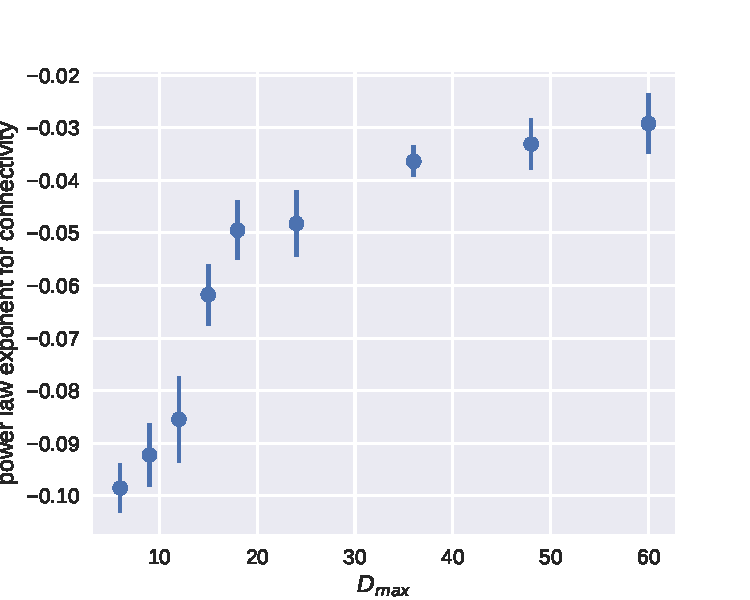
\includegraphics[width=0.95\columnwidth]{pics/instances/connectivity_pl.pdf}
  \caption{\label{fig:pl_cc}(Left) Histogram of the connectivity, regardless the
  connected component, at fixed maximum delay time of $60$ minutes. As one can see, the
  connectivity follows a power-law distribution. The coefficient of this
  power-law depends on the maximum delay time. (Right) coefficients of the
  power-law distribution by varying the maximum delay time.}
\end{figure*}

Even though the connectivity gives already an indication of the underlying
structure of the topology of the conflict graph, it cannot be used to determine
whether the graph has a tree-like structure or not. Indeed, if a connected
component of the conflict graph were a tree, an optimal solution can be
trivially found by iteratively propagate the delays along the tree. On the
contrary, if flights in a connected components form a fully-connected graph
(namely, all flights have pairwise potential conflicts), an optimal solution is
hard to find. In order to understand if the connected components of the conflict
graph look like tree, we studied the treewidth of the connected
components \cite{bertele1972, halin1976s}.\\

Intuitively, the treewidth is a property of a given graph and its value ranges
from 1 (the graph is a tree) to the size of the graph (the graph is
fully-connected). As shown in Figure~(\ref{fig:hist_tw}), large parte of the
connected components have a tree-like shape while few connected components (the
hardest to find an optimal solution) look more like a fully-connected graph.

\begin{figure}
  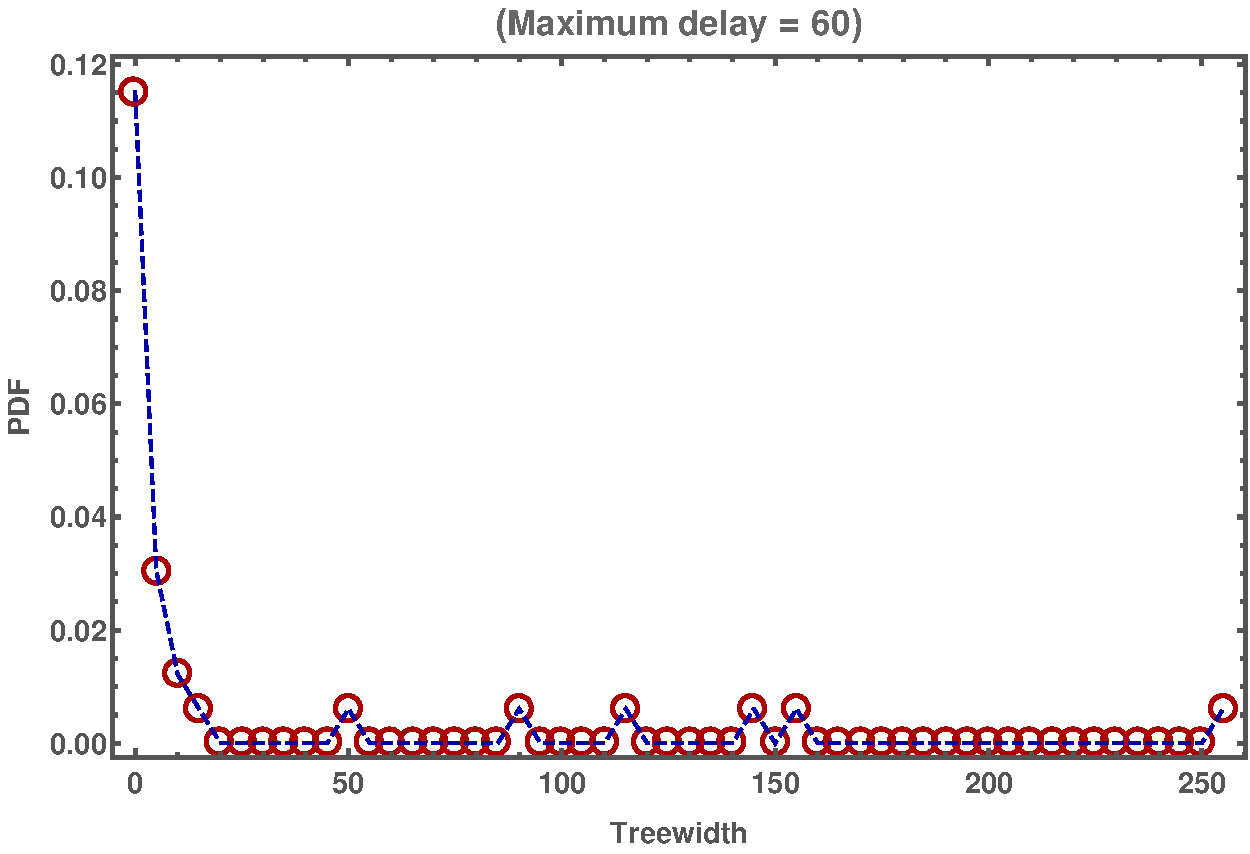
\includegraphics[width=\columnwidth]{pics/instances/treewidth_histogram.pdf}
  \caption{\label{fig:hist_tw}Histogram of the treewidth of a given connected
  component, regardless the maximum delay time.}
\end{figure}

To be more precise, left panel of Figure~(\ref{fig:tw_vs_cc}) shows how the
treewidth scales with the number of flights inside a given connected component.
It is interesting to observe that the treewidth increases linearly with the
number of flights belonging to the given connected component. This implies that
larger connected components are also the hardest to optimize. Moreover, the
slope $\gamma$ of the linear correlation between the size of the connected
components and their treewidth increases by increasing the maximum delay time
(see right panel of Figure~(\ref{fig:tw:vs:cc}). This is consistent with the
idea that preprocessing the flight dataset with a given maximum delay time makes
indeed the ATM problem easier to tackle.

\begin{figure*}
  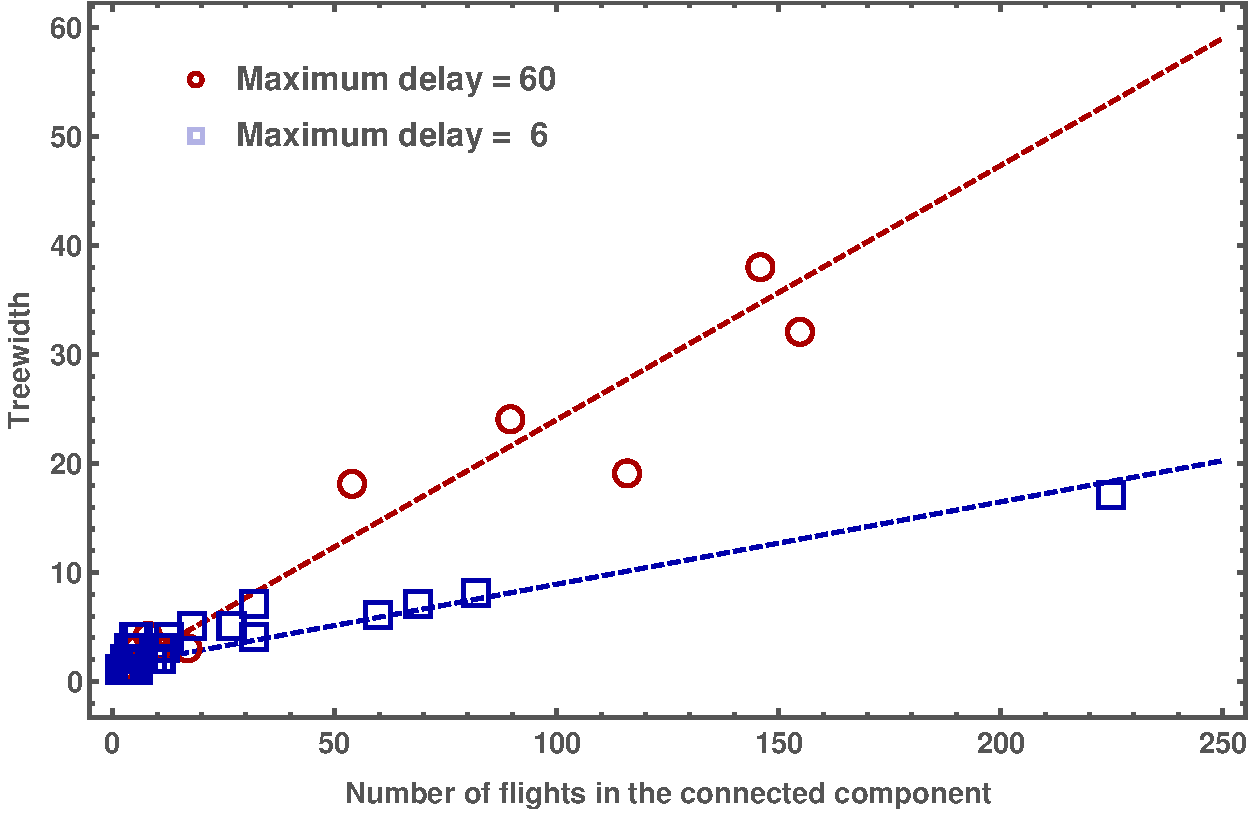
\includegraphics[width=\columnwidth]{pics/instances/treewidth_connectivity.pdf}
  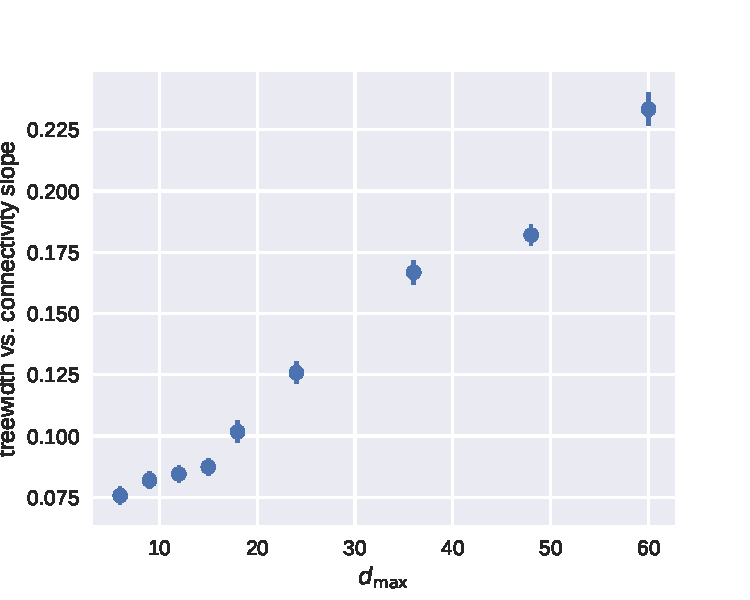
\includegraphics[width=\columnwidth]{pics/instances/treewidth_pl.pdf}
  \caption{\label{fig:tw_vs_cc}(Left) Figure shows how the treewidth of a given
  connected component as a function of the number of flights. Interestingly, the
  treewidth is linear with the number of flights, with a slope $\gamma$ which
  depends the on the maximum delay time. (Right) Slope $\gamma$ as a function
  of the maximum delay time.}
\end{figure*}


